\documentclass[tikz]{standalone}

\usepackage[latin1]{inputenc}
\usepackage{tikz}

% GNUPL
\begin{document}
\pagestyle{empty}


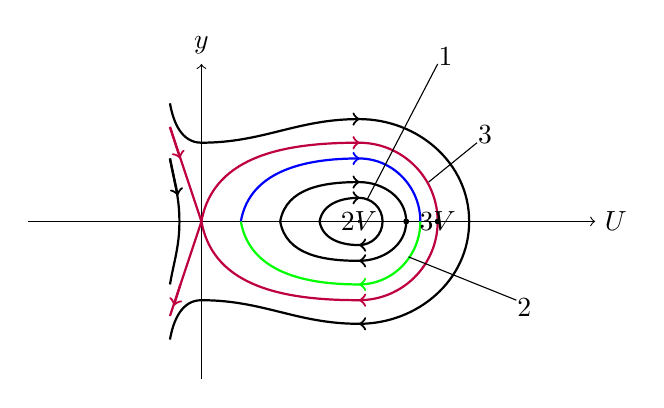
\begin{tikzpicture}
    %\draw[very thin,color=gray] (-1,1.1) grid (3.9,3.9);
    \draw[->] (-2.2,0) -- (5,0) node[right] {$U$};
    \draw[->] (0,-2) -- (0,2) node[above] {$y$};
	%фокус(-покус)
    \draw[purple,thick] (0,0) to [out=80,in=180] (2,1);
    \draw[purple,thick] (2,1) to [out=0,in=90] (3,0);
    \draw[purple,thick] (0,0) to [out=-80,in=180] (2,-1);
    \draw[purple,thick] (2,-1) to [out=0,in=-90] (3,0);
    \draw[purple,thick] [->] (2,1) --(2.01,1);
    \draw[purple,thick] [<-] (2,-1) --(2.01,-1);
    \coordinate [label=center:$3$] (3) at (3.6,1.1);
    \draw (3.5,1) -- (2.885,0.5);
    

    \draw[blue,thick] (0.5,0) to [out=80,in=180] (2,0.8);
    \draw[blue, thick] (2,0.8) to [out=0,in=90] (2.78,0);
    \draw[green, thick] (0.5,0) to [out=-80,in=180] (2,-0.8);
    \draw[green, thick] (2,-0.8) to [out=0,in=-90] (2.78,0);
    \draw[blue,thick] [->] (2,0.8) --(2.01,0.8);
    \draw[green, thick] [<-] (2,-0.8) --(2.01,-0.8);

    \draw[thick] (1,0) to [out=80,in=180] (2,0.5);
    \draw[thick] (2,0.5) to [out=0,in=90] (2.6,0);
    \draw[thick] (1,0) to [out=-80,in=180] (2,-0.5);
    \draw[thick] (2,-0.5) to [out=0,in=-90] (2.6,0);
    \draw[thick] [->] (2,0.5) --(2.01,0.5);
    \draw[thick] [<-] (2,-0.5) --(2.01,-0.5);
    \coordinate [label=center:$2$] (2) at (4.1,-1.1);
    \draw (4,-1) -- (2.63,-0.45);


    \draw[thick] (1.5,0) to [out=80,in=180] (2,0.3);
    \draw[thick] (2,0.3) to [out=0,in=90] (2.3,0);
    \coordinate [label=center:$1$] (1) at (3.1,2.1);
    \draw (3,2) -- (2.1,0.27);
    \draw[thick] (1.5,0) to [out=-80,in=180] (2,-0.3);
    \draw[thick] (2,-0.3) to [out=0,in=-90] (2.3,0);
    \draw[thick] [->] (2,0.3) --(2.01,0.3);
    \draw[thick] [<-] (2,-0.3) --(2.01,-0.3);
	%седло
	\draw[purple, thick] (-0.4,1.2) -- (0,0);
	\draw[purple,thick] (-0.4,-1.2) -- (0,0);
	\draw[thick] (-0.4,0.8) to [out=-80,in=90] (-0.28,0);
	\draw[thick] (-0.4,-0.8) to [out=80,in=-90] (-0.28,0);
	\draw[thick] [->]  (-0.4,0.8) -- (-0.3,0.33);
	\draw[purple,thick] [->] (-0.4,1.2) --(-0.27,0.8);
	\draw[purple,thick] [<-] (-0.35,-1.07) --(-0.268,-0.8);
	%не имеющие физ смысла
	\draw[thick] (-0.4,1.5) to [out=-80,in=180] (0,1);
	\draw[thick] (0,1) to [out=0,in=-180] (2,1.3);
	\draw[thick] (2,1.3) to [out=0,in=90] (3.4,0);
	\draw[thick] (-0.4,-1.5) to [out=80,in=180] (0,-1);
	\draw[thick] (0,-1) to [out=0,in=-180] (2,-1.3);
	\draw[thick] (2,-1.3) to [out=0,in=-90] (3.4,0);
	\draw[thick] [->] (2,1.3) --(2.01,1.3);
	\draw[thick] [<-] (2,-1.3) --(2.01,-1.3);

    % \coordinate [label=center:$1$] (1) at (1,0);
    \coordinate [label=center:$2V$] (2V) at (2,0);
    \coordinate [label=center:$3V$] (3V) at (3,0);
    \draw [fill] (2,0) circle [radius=0.01];
    \draw [fill] (2.6,0) circle [radius=0.03];
    \draw [fill] (3,0) circle [radius=0.03];
\end{tikzpicture}


\end{document}